\hypertarget{ontwerpen-en-printen}{%
\section{Ontwerpen en printen}\label{ontwerpen-en-printen}}

De meest voor de hand liggende optie voor ons was Tinkercad.\footnote{https://tinkercad.com}
Dit is een webapplicatie en hierdoor op elke computer met een
internetverbinding te gebruiken. Het ontwerpen gaat door bepaalde vormen
aan je document toe te voegen en die te vervormen. Bepaalde vormen
kunnen ook in negatieve stand, waardoor die vorm uit de andere vorm
gehaald kan worden.

\begin{figure}
\centering
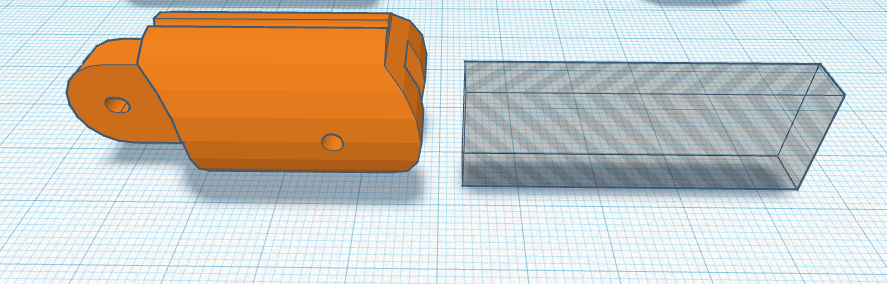
\includegraphics[width=0.72\textwidth,height=\textheight]{img/image_17.png}
\caption{Normale en negatieve vorm\label{fig:tinkercad}}
\end{figure}

Voor het printen hebben wij de MakerBot Replicator
(\xrefname{Fig.}\cref{fig:makerbot}) gebruikt. Dit is een desktop
3d-printer met een applicatie voor de Mac. Bij deze printer zijn er heel
veel instellingen te veranderen, iets dat wij dan ook uitgebreid hebben
gedaan. Hiervoor hadden wij een preset gemaakt waarin instellingen zoals
de laagdikte, reissnelheid van de kop, printtemperatuur en dikte
ondersteuningsstructuur ingesteld staan.

\begin{figure}
\centering
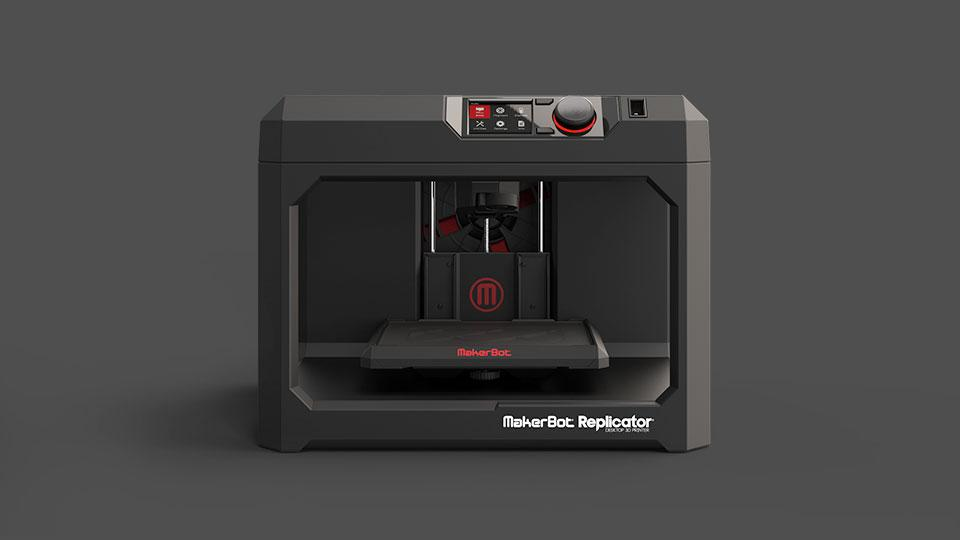
\includegraphics[width=0.55\textwidth,height=\textheight]{img/image_18.jpg}
\caption{De Makerbot Replicator\label{fig:makerbot}}
\end{figure}

In de loop van de tijd zijn wij meerdere problemen tegengekomen in het
ontwerp, deze hebben we telkens opgelost door zowel grote als kleine
aanpassingen te maken. Zo had de eerste versie van de vinger nog geen
ruimte in de binnenkant voor de mechaniek (het visdraad). Dit proces is
geïllustreerd in \xrefname{Fig.}\cref{fig:middenkootje}.

Bij het ontwerp hebben we ook rekening gehouden met de verhouding van
Fibonacci uit sectie §3.4. Door deze reeks te gebruiken hebben we
geprobeerd een hand te maken die zoveel mogelijk overeenkomt met een
normale mensenhand.

\begin{figure}
\centering
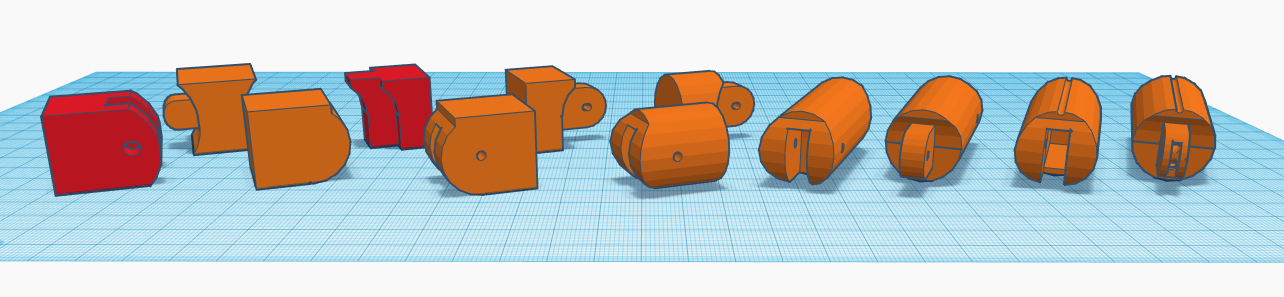
\includegraphics[width=1\textwidth,height=\textheight]{img/image_19.png}
\caption{Proces van het ontwerpen van het
middenkootje\label{fig:middenkootje}}
\end{figure}

Op de plek waar alle vingers bij elkaar komen, de handpalm, trad een
nieuw probleem op. Je kan immers niet de binnenste twee vingers
vastzetten, aangezien het koppelstuk van de buitenste twee vingers
hierbij in de weg zat. Om deze twee te kunnen plaatsen moesten wij een
schuifmechanisme bedenken dat stevig genoeg zou zijn dat het niet los
zou schieten, maar ook makkelijk te verwijderen is, aangezien je alleen
op deze manier de vingers aan de knokkels vast kon maken met een pin.

\begin{figure}
\centering
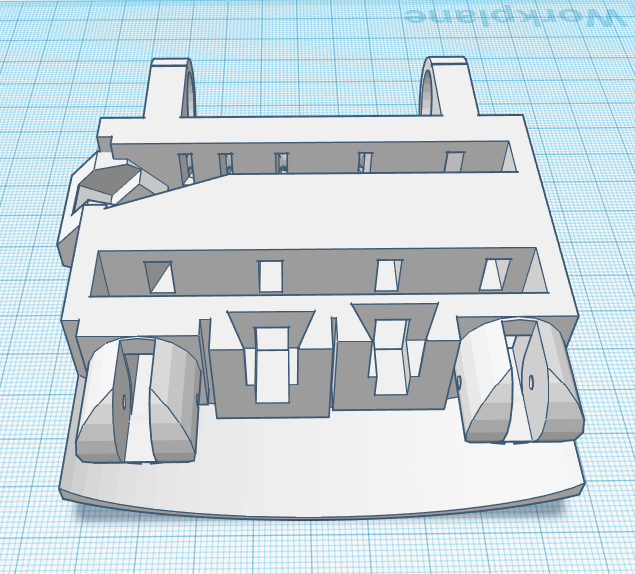
\includegraphics[width=0.44\textwidth,height=\textheight]{img/image_20.png}
\caption{Palm van onderen met vertoning
knokkelschuifjes\label{fig:palm}}
\end{figure}

In \xrefname{Fig.}\cref{fig:palm} kun je zien dat de vingers met
pinnetjes aan de knokkels vast worden gemaakt en dat dat niet mogelijk
zou zijn bij de ring- en middelvinger als deze niet verwijderd konden
worden.
